\documentclass[a4paper,12pt]{report}
\usepackage{titlesec}
\usepackage{amssymb}
\usepackage{amsmath}
\usepackage{graphicx}
\usepackage{geometry}
\geometry{a4paper,left=25mm,right=25mm,top=30mm,bottom=30mm}
\usepackage{cite}
\usepackage{tikz}
\usetikzlibrary{arrows.meta, positioning, shapes.geometric, calc}
\usepackage{titlesec}
\titleformat{\chapter}[display]
  {\normalfont\huge\bfseries\centering}
  {\chaptertitlename\ \thechapter}{20pt}{\Huge}

\begin{document}
\thispagestyle{empty}
\begin{center}
 \huge{\textsc{RTL Design of a KCF Visual Tracker}}
\end{center}
\vspace{0.25cm}
\begin{center}
 \LARGE{Spring 2026}
\end{center}
\vspace{0.5cm}
\begin{center}
 \large{Submitted by}
\end{center}
\vspace{0.5cm}
\begin{center}
 \large{Akhil Sriram (Roll No. [Insert Roll No.])}\\
\end{center}
 \vspace{0.25cm}
\begin{center}
 \large{Under Supervision of}
\end{center}
\vspace{0.25cm}
\begin{center}
 \large{Dr. Venkatnarayan Hariharan}\\
 \large{Department of Electrical Engineering}\\
\end{center}
\begin{figure}[htbp]
	\centering
		
\includegraphics[width=4in]{logo.jpg}
\end{figure}
\vspace{0.25cm}
\begin{center}
\large{\textbf{Department of Electrical Engineering}}\\
\large{\textbf{School of Engineering}}\\
\large{\textbf{Shiv Nadar University}}\\
\vspace{0.25cm}
(Spring 2026)
\end{center}
\pagebreak
\begin{center}
\huge{\textsc{Abstract}}
\end{center}
Visual object tracking is a computationally demanding task in computer vision, typically requiring high-performance CPUs or GPUs to maintain real-time frame rates. This project presents a Register Transfer Level (RTL) implementation of the Kernelized Correlation Filter (KCF) algorithm, designed to accelerate the tracking pipeline using dedicated FPGA hardware. For this mid-semester Minimum Viable Product (MVP), the architecture is specifically optimized for the detection phase: operating on a scaled-down 32$\times$32 pixel patch, utilizing a linear kernel to bypass complex exponential calculations, and loading offline-trained filter coefficients ($\hat{\alpha}$) from static memory. The pipelined hardware integrates a custom 2D Fast Fourier Transform (FFT) core, element-wise conjugate multiplication, 2D Inverse FFT (IFFT), and a spatial peak detection module. The design has been verified through behavioral simulation in both Icarus Verilog and Xilinx Vivado, with the hardware output matching the Python golden reference exactly.

\pagebreak
\tableofcontents
\pagebreak
\listoffigures
\pagebreak
\chapter{Introduction}
\section{Background and Motivation}
Real-time visual tracking is a fundamental component in robotics, autonomous navigation, and smart surveillance systems. The primary challenge in these domains is tracking a fast-moving Region of Interest (ROI) with minimal latency and low power consumption. Software-based implementations often struggle to meet these strict timing constraints without relying on power-hungry processors.

By translating the tracking algorithm into a custom hardware accelerator (IP core), we can achieve cycle-accurate, highly parallelized execution, drastically reducing the time required to process each incoming video frame.

\section{The KCF Advantage}
Traditional spatial-domain tracking algorithms rely on sliding a template across a search window and computing metrics like Sum of Absolute Differences (SAD) or Normalized Cross-Correlation (NCC). This approach is highly inefficient, as the time complexity scales quadratically with the image size.

The Kernelized Correlation Filter (KCF) \cite{henriques2015} elegantly sidesteps this bottleneck. By leveraging the properties of circulant matrices, KCF transforms the image patch into the frequency domain using a 2D Fast Fourier Transform (2D-FFT). In the frequency domain, massive spatial convolutions are reduced to simple element-wise multiplications, allowing for immense computational speedups when mapped to hardware.

\section{Scope of the Mid-Semester MVP}
To demonstrate the viability of the hardware approach within the mid-semester timeline, the following simplifications were adopted:
\begin{itemize}
    \item \textbf{32$\times$32 patch size} instead of the full 64$\times$64, reducing memory and FFT complexity by 4$\times$.
    \item \textbf{Linear kernel} instead of a Gaussian kernel, eliminating the need for a hardware exponential function.
    \item \textbf{Detection only}: the model is trained offline in Python and the frozen filter coefficients ($\hat{\alpha}$) are loaded from ROM. The online model update loop is deferred to the next phase.
    \item \textbf{No AXI bus interface}: pixels are loaded directly via a simple write port for simulation.
\end{itemize}

\chapter{Literature Survey}
\section{Correlation Filters in Computer Vision}
The shift from spatial to frequency-domain tracking gained significant traction with the introduction of Minimum Output Sum of Squared Error (MOSSE) filters \cite{bolme2010}, which later evolved into KCF. KCF improved upon its predecessors by introducing the ``Kernel Trick,'' allowing the filter to map features into a higher-dimensional space for better target separation, while maintaining the speed advantages of the FFT \cite{henriques2015}.

\section{Hardware Acceleration of the FFT}
The critical path in any KCF hardware implementation is the Fourier Transform. Efficient RTL designs utilize the Cooley-Tukey algorithm \cite{cooleytukey1965}, specifically the Radix-2 Decimation-In-Time (DIT) architecture. By iteratively passing data through Butterfly units, the mathematical complexity is reduced from $O(N^2)$ to $O(N \log N)$, making it viable for synthesizable logic.

\chapter{Work Done}
\section{Algorithm Pipeline Overview}
The KCF algorithm consists of two primary stages: the \textbf{Training Stage} (updating the model) and the \textbf{Tracking Stage} (detecting the target). Figure~\ref{f_kcf_overview} illustrates this high-level workflow.

For the mid-semester MVP, the focus is entirely on accelerating the \textbf{Tracking Stage}. To isolate and verify the detection math, the model update phase is bypassed by training the model offline in Python and loading the frozen $\hat{\alpha}$ coefficients from a \texttt{.mem} file.

\begin{figure}[ht]
\centering
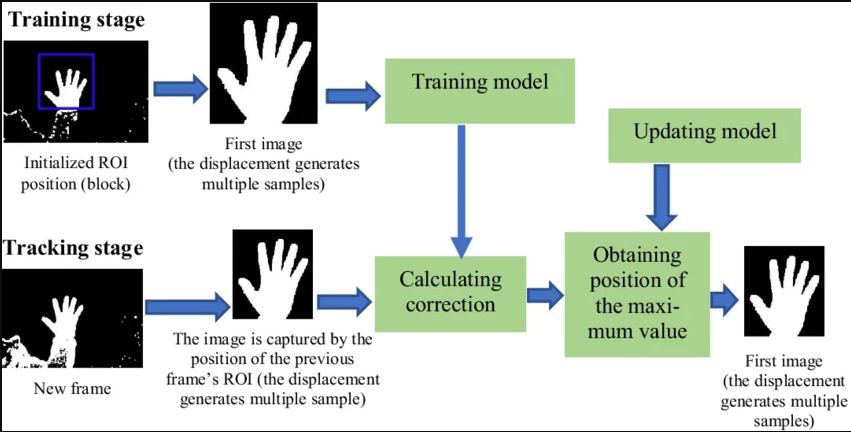
\includegraphics[width=5in]{KCF.png}
\caption{High-level overview of the KCF algorithm showing both the training and tracking stages. The training stage learns the filter model from an initial frame, while the tracking stage uses it to locate the target in subsequent frames.}
\label{f_kcf_overview}
\end{figure}

\section{Detection Pipeline}
The core of this project is the hardware detection pipeline. Given a new image patch and pre-trained filter coefficients $\hat{\alpha}$, the pipeline computes the response map and finds the peak location, which corresponds to the estimated target displacement. The mathematical flow is:
\begin{equation}
\text{response} = \text{IFFT}\left(\overline{\hat{\alpha}} \odot \text{FFT}(\text{patch} \cdot w)\right)
\label{eq_detect}
\end{equation}
where $w$ is the 2D Hann window, $\odot$ denotes element-wise multiplication, and the overline denotes complex conjugation. The peak of the response map gives the (row, col) displacement of the target from its expected position.

Figure~\ref{f_pipeline} shows the block-level view of the hardware detection pipeline.

\begin{figure}[ht]
\centering
\resizebox{\textwidth}{!}{%
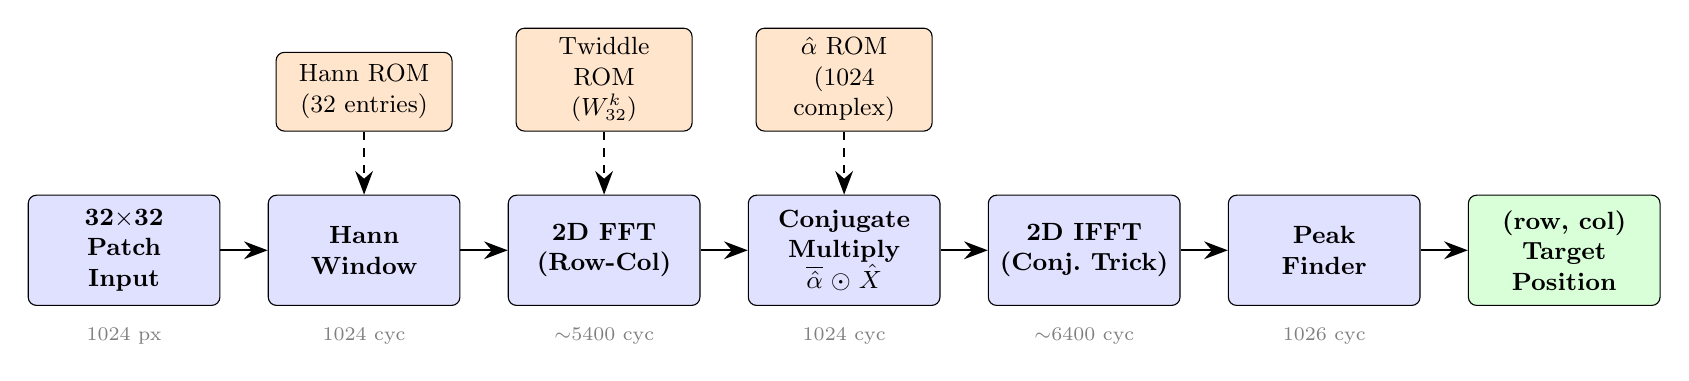
\begin{tikzpicture}[
    block/.style={rectangle, draw, fill=blue!12, text width=2.2cm, minimum height=1.4cm, align=center, font=\small\bfseries, rounded corners=3pt},
    rom/.style={rectangle, draw, fill=orange!20, text width=2cm, minimum height=1cm, align=center, font=\small, rounded corners=3pt},
    data/.style={-{Stealth[length=3mm]}, thick},
    label/.style={font=\scriptsize, text=gray},
    node distance=0.6cm
]
    % Main pipeline blocks
    \node[block] (input) {32$\times$32\\Patch\\Input};
    \node[block, right=of input] (hann) {Hann\\Window};
    \node[block, right=of hann] (fft) {2D FFT\\(Row-Col)};
    \node[block, right=of fft] (mul) {Conjugate\\Multiply\\$\overline{\hat{\alpha}} \odot \hat{X}$};
    \node[block, right=of mul] (ifft) {2D IFFT\\(Conj.\ Trick)};
    \node[block, right=of ifft] (peak) {Peak\\Finder};
    \node[block, right=of peak, fill=green!15] (out) {(row, col)\\Target\\Position};

    % ROM blocks
    \node[rom, above=0.8cm of hann] (hannrom) {Hann ROM\\(32 entries)};
    \node[rom, above=0.8cm of mul] (alpharom) {$\hat{\alpha}$ ROM\\(1024 complex)};
    \node[rom, above=0.8cm of fft] (twrom) {Twiddle ROM\\($W_{32}^k$)};

    % Data flow arrows
    \draw[data] (input) -- (hann);
    \draw[data] (hann) -- (fft);
    \draw[data] (fft) -- (mul);
    \draw[data] (mul) -- (ifft);
    \draw[data] (ifft) -- (peak);
    \draw[data] (peak) -- (out);

    % ROM arrows
    \draw[data, dashed] (hannrom) -- (hann);
    \draw[data, dashed] (alpharom) -- (mul);
    \draw[data, dashed] (twrom) -- (fft);

    % Stage labels below
    \node[label, below=0.15cm of input] {1024 px};
    \node[label, below=0.15cm of hann] {1024 cyc};
    \node[label, below=0.15cm of fft] {$\sim$5400 cyc};
    \node[label, below=0.15cm of mul] {1024 cyc};
    \node[label, below=0.15cm of ifft] {$\sim$6400 cyc};
    \node[label, below=0.15cm of peak] {1026 cyc};

\end{tikzpicture}
}%
\caption{Hardware detection pipeline block diagram. Data flows left to right through seven stages controlled by a central FSM. Dashed arrows indicate pre-computed data loaded from ROM. The cycle counts show the latency of each stage at the system clock.}
\label{f_pipeline}
\end{figure}

\section{System Architecture and FSM}
The top-level module, \texttt{kcf\_detect\_top.sv}, orchestrates a 7-stage Finite State Machine (FSM) that processes the patch sequentially:
\begin{enumerate}
    \item \textbf{S\_HANN\_WIN} (1024 cycles): Applies a 2D Hann window to the incoming 32$\times$32 image patch. The Hann window smoothly tapers the edges of the patch to zero, preventing sharp discontinuities that would create misleading high-frequency artifacts in the FFT output. The 2D window is computed as the outer product of two 1D Hann vectors, with the coefficients stored in ROM.
    \item \textbf{S\_FFT\_LOAD} (1024 cycles): Loads the windowed patch into the 2D FFT module's internal buffer, one pixel per clock cycle.
    \item \textbf{S\_FFT\_RUN} ($\sim$5400 cycles): Computes the 2D FFT to bring the spatial-domain image data into the frequency domain. Internally, this processes 32 rows and then 32 columns, each requiring $\sim$83 clock cycles.
    \item \textbf{S\_ELEM\_MUL} (1024 cycles): Performs element-wise conjugate multiplication between the FFT of the patch ($\hat{X}$) and the stored filter coefficients ($\hat{\alpha}$). This step replaces the expensive spatial convolution with a simple multiply.
    \item \textbf{S\_IFFT\_LOAD} (1024 cycles): Loads the resulting frequency-domain product into the 2D IFFT module.
    \item \textbf{S\_IFFT\_RUN} ($\sim$6400 cycles): Computes the 2D Inverse FFT to transform the product back into the spatial domain, producing the response map.
    \item \textbf{S\_PEAK\_RUN} (1026 cycles): Scans the entire response map sequentially to find the pixel with the maximum value. The row and column of this peak are the final tracking output.
\end{enumerate}
The total detection latency is approximately \textbf{19,300 clock cycles}. At a 100\,MHz system clock, this corresponds to $\sim$193\,$\mu$s per frame.

\section{Key Building Blocks}

\subsection{The Butterfly Unit}
The butterfly is the atomic computation of the FFT. Named for the shape of its signal-flow diagram, it takes two complex inputs ($a$ and $b$) along with a pre-computed rotation factor called a \textit{twiddle factor} ($W$), and produces two outputs:
\begin{align}
    \text{out}_a &= a + W \cdot b \\
    \text{out}_b &= a - W \cdot b
\end{align}
This operation is entirely combinational in our design and completes in a single clock cycle. To prevent numerical overflow during successive additions, a \textit{scaled} variant divides both outputs by 2 (implemented as a single-bit arithmetic right shift \texttt{>>>~1}).

\subsection{Twiddle Factors}
Twiddle factors are the ``rotation angles'' that the FFT uses to decompose a signal into its frequency components. For a 32-point FFT, they are defined as:
\begin{equation}
    W_{32}^k = e^{-j \cdot 2\pi k / 32} = \cos\!\left(\frac{2\pi k}{32}\right) - j\sin\!\left(\frac{2\pi k}{32}\right), \quad k = 0, 1, \ldots, 15
\end{equation}
These 16 complex values are pre-computed in Python and stored in a ROM (\texttt{twiddle\_rom\_32.sv}), with real and imaginary parts interleaved. The symmetry property $W^{k+N/2} = -W^k$ means only half the values need to be stored.

\subsection{1D FFT (32-Point)}
The 32-point 1D FFT (\texttt{fft1d\_32.sv}) uses an iterative single-butterfly architecture based on the Cooley-Tukey Radix-2 Decimation-In-Time (DIT) algorithm. The key steps are:
\begin{enumerate}
    \item \textbf{Bit-Reversal Permutation:} The 32 input samples are reordered by reversing their 5-bit binary indices (e.g., index 3 = \texttt{00011} maps to index 24 = \texttt{11000}). This reordering allows the subsequent butterfly stages to operate on adjacent memory locations.
    \item \textbf{5 Butterfly Stages:} Each stage performs 16 butterfly operations. The ``distance'' between butterfly pairs doubles at each stage (1, 2, 4, 8, 16), progressively combining more of the input data.
    \item \textbf{Total:} $5 \times 16 = 80$ butterfly operations $+$ overhead $\approx 83$ clock cycles per 1D transform.
\end{enumerate}

\subsection{2D FFT (Row-Column Decomposition)}
The 2D FFT (\texttt{fft2d\_32.sv}) decomposes the 2D transform into two passes of 1D transforms:
\begin{enumerate}
    \item \textbf{Row Pass:} Apply the 1D FFT to each of the 32 rows (with scaling enabled to prevent overflow).
    \item \textbf{Column Pass:} Apply the 1D FFT to each of the 32 columns of the row-transformed result (without scaling, to preserve signal magnitude).
\end{enumerate}
This asymmetric scaling strategy (rows scaled, columns unscaled) was critical to solving the fixed-point precision challenge, as discussed in Section~\ref{sec_fixedpoint}.

\subsection{2D IFFT (Conjugate Trick)}
Computing an inverse FFT from scratch would require a separate hardware module. Instead, the IFFT is implemented by reusing the same FFT hardware through the \textit{conjugate trick}:
\begin{equation}
    \text{IFFT}(X) = \overline{\text{FFT}(\overline{X})} \;/\; N^2
\end{equation}
The steps are: (1)~negate all imaginary parts of the input (conjugate), (2)~run the forward FFT, (3)~negate all imaginary parts of the output (conjugate again). The $1/N^2$ normalization is handled automatically by the scaled butterfly architecture.

\section{Fixed-Point Arithmetic}
\label{sec_fixedpoint}
All computations use Q8.8 fixed-point representation: 16-bit signed values with 8 integer bits and 8 fractional bits. This format can represent values from $-128$ to $+127.996$ with a resolution of $1/256 \approx 0.004$.

\subsection{The Scaling Challenge}
A significant engineering challenge was maintaining adequate signal precision through the pipeline. With the 2D FFT applying a scaling factor of $1/N$ per butterfly stage across both row and column passes, the total attenuation was $1/N^2 = 1/1024$. This caused the final response values to fall below the smallest representable Q8.8 value, effectively rounding everything to zero.

The solution combined two techniques:
\begin{itemize}
    \item \textbf{Asymmetric FFT scaling:} The forward FFT scales only the row pass (dividing by $N=32$), while leaving the column pass unscaled. The IFFT uses full scaling on both passes for correct normalization. This reduces the total attenuation from $1/N^2$ to $1/N$.
    \item \textbf{Alpha pre-scaling:} The filter coefficients $\hat{\alpha}$ are multiplied by a factor of $K=16$ during the offline Python generation step. This further compensates for the remaining $1/N$ factor, yielding a final pipeline output of $(K/N) \times \text{response} = 0.5 \times \text{response}$, comfortably within the Q8.8 dynamic range.
\end{itemize}

\chapter{Results and Verification}
\section{Simulation Environment}
The design was verified in two independent simulation environments:
\begin{itemize}
    \item \textbf{Icarus Verilog (iverilog):} Used for rapid iterative development and debugging during the implementation phase.
    \item \textbf{Xilinx Vivado 2024.2:} Used for final verification with the target FPGA toolchain.
\end{itemize}

A Python script (\texttt{gen\_data\_32.py}) generates all test data and computes the golden reference. The test patch consists of a 32$\times$32 image with a uniform background (intensity 0.1) and a bright 5$\times$5 square feature centred at pixel (18, 20). The offline-trained filter coefficients produce a golden detection peak at row~18, column~19.

\section{Vivado Waveform Analysis}
Figure~\ref{f_wave_full} shows the complete simulation waveform from Vivado. The pipeline processes the patch through all seven FSM stages, completing in approximately 193\,$\mu$s. The final output signals \texttt{peak\_row} and \texttt{peak\_col} transition from undefined (\texttt{XX}) to their correct values at the moment the \texttt{done} signal pulses high.

\begin{figure}[ht]
\centering
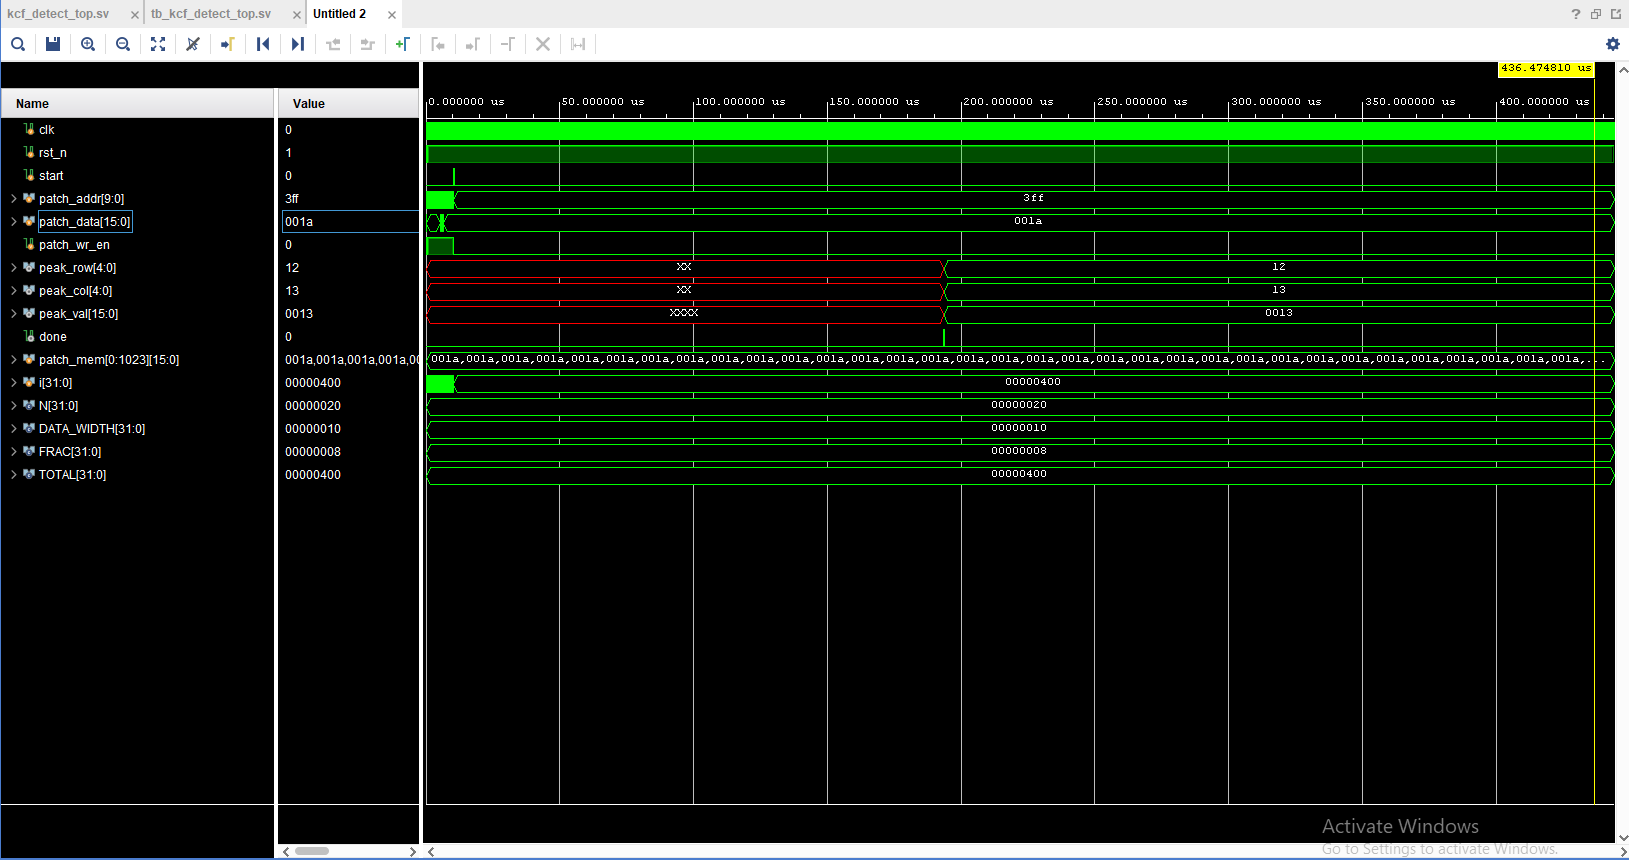
\includegraphics[width=\textwidth]{waveform.png}
\caption{Full Vivado simulation waveform showing the complete detection pipeline execution. The patch is loaded during the first $\sim$5\,$\mu$s, followed by windowing, FFT, multiplication, IFFT, and peak finding stages.}
\label{f_wave_full}
\end{figure}

Figure~\ref{f_wave_zoom} zooms into the critical moment at $\sim$193,465\,ns where the pipeline produces its final result. The \texttt{done} signal pulses high for exactly one clock cycle, and the outputs latch to their final values:
\begin{itemize}
    \item \texttt{peak\_row} = \texttt{0x12} = \textbf{18} (decimal)
    \item \texttt{peak\_col} = \texttt{0x13} = \textbf{19} (decimal)
    \item \texttt{peak\_val} = \texttt{0x0013} = 19 (decimal) = $19/256 = 0.074$ in Q8.8
\end{itemize}
These values match the Python golden reference exactly, confirming correct end-to-end operation of the hardware pipeline.

\begin{figure}[ht]
\centering
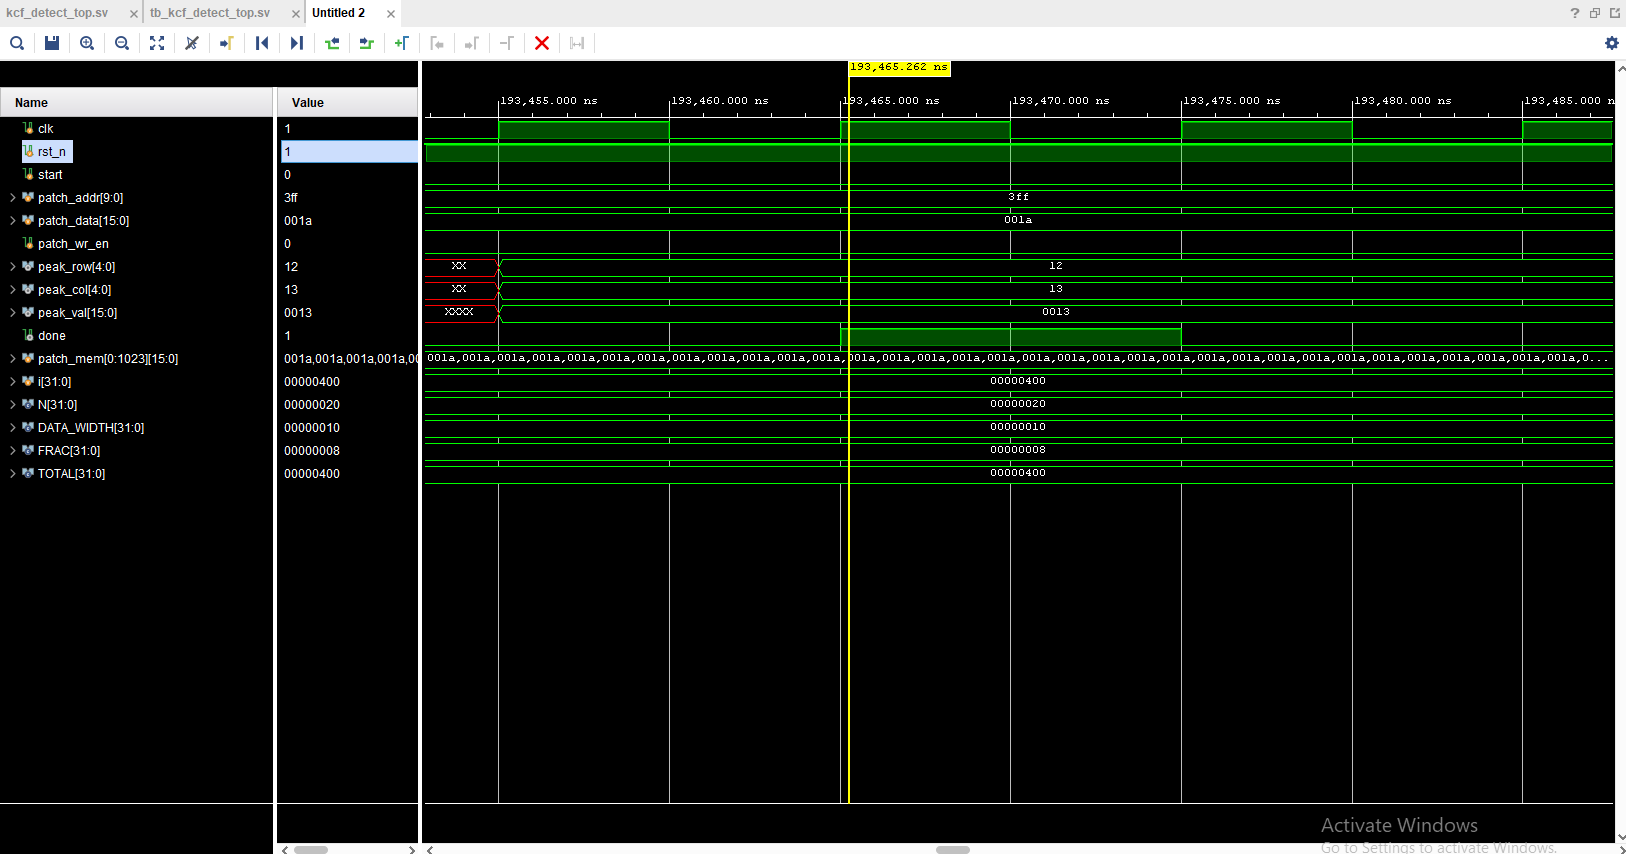
\includegraphics[width=\textwidth]{zoomed in.png}
\caption{Zoomed-in view of the simulation output at $t \approx 193,465$\,ns. The \texttt{done} pulse (highlighted) coincides with the outputs settling to \texttt{peak\_row}~=~18, \texttt{peak\_col}~=~19, matching the golden reference.}
\label{f_wave_zoom}
\end{figure}

\chapter{Future Work}
\section{Next Objectives}
With the baseline detection pipeline functioning correctly in simulation, the next phase of the project will focus on scaling the architecture and integrating it into a full System-on-Chip (SoC) environment:
\begin{enumerate}
    \item \textbf{Hardware Deployment:} Synthesize and deploy the verified RTL logic onto the Xilinx Artix-7 FPGA to evaluate real-world timing and resource consumption.
    \item \textbf{Resolution Scaling:} Expand the FFT modules to support $64 \times 64$ patches. This will require adding a 6th FFT stage and quadrupling the memory buffer sizes.
    \item \textbf{Kernel Upgrade:} Transition from a simple linear kernel to a Gaussian kernel, which will necessitate the implementation of a hardware exponential approximation Look-Up Table (LUT).
    \item \textbf{Online Model Updating:} Implement the mathematical logic to dynamically update the $\hat{\alpha}$ filter coefficients live, allowing the tracker to adapt to changing target appearances (e.g., rotations or lighting changes) rather than relying on frozen offline data.
    \item \textbf{AXI Bus Integration:} Wrap the KCF tracking core in an AXI4-Stream interface to seamlessly accept high-bandwidth, continuous pixel data from the SoC's Direct Memory Access (DMA) controller.
\end{enumerate}

\pagebreak
\addcontentsline{toc}{section}{References}
\bibliographystyle{IEEEtran}
\bibliography{reference}

\end{document}
